\documentclass[12pt]{article}
\usepackage[left=1cm, right=1cm, top=2cm,bottom=1.5cm]{geometry} 

\usepackage[parfill]{parskip}
\usepackage[utf8]{inputenc}
\usepackage[T2A]{fontenc}
\usepackage[russian]{babel}
\usepackage{enumitem}
\usepackage[normalem]{ulem}
\usepackage{amsfonts, amsmath, amsthm, amssymb, mathtools}
\usepackage{tabularx}
\usepackage{hhline}

\usepackage{accents}
\usepackage{fancyhdr}
\pagestyle{fancy}
\renewcommand{\headrulewidth}{1.5pt}
\renewcommand{\footrulewidth}{1pt}

\usepackage{graphicx}
\usepackage[figurename=Рис.]{caption}
\usepackage{subcaption}
\usepackage{float}

%%Наименование папки откуда забирать изображения
\graphicspath{ {./images/} }

%%Изменение формата для ввода доказательства
\renewcommand{\proofname}{$\square$  \nopunct}
\renewcommand\qedsymbol{$\blacksquare$}

%%Изменение отступа на таблицах
\addto\captionsrussian{%
	\renewcommand{\proofname}{$\square$ \nopunct}%
}
%% Римские цифры
\newcommand{\RN}[1]{%
	\textup{\uppercase\expandafter{\romannumeral#1}}%
}

%% Для удобства записи
\newcommand{\MR}{\mathbb{R}}
\newcommand{\MQ}{\mathbb{Q}}
\newcommand{\MN}{\mathbb{N}}
\newcommand{\MI}{\mathrm{I}}
\newcommand{\MJ}{\mathrm{J}}
\newcommand{\MH}{\mathrm{H}}
\newcommand{\MT}{\mathrm{T}}
\newcommand{\MU}{\mathcal{U}}
\newcommand{\MV}{\mathcal{V}}
\newcommand{\VN}{\varnothing}
\newcommand{\VE}{\varepsilon}

\theoremstyle{definition}
\newtheorem{defn}{Опр:}
\newtheorem{rem}{Rm:}
\newtheorem{prop}{Утв.}
\newtheorem{exrc}{Упр.}
\newtheorem{lemma}{Лемма}
\newtheorem{theorem}{Теорема}
\newtheorem{corollary}{Следствие}

\newenvironment{cusdefn}[1]
{\renewcommand\thedefn{#1}\defn}
{\enddefn}

\DeclareRobustCommand{\divby}{%
	\mathrel{\text{\vbox{\baselineskip.65ex\lineskiplimit0pt\hbox{.}\hbox{.}\hbox{.}}}}%
}
%Короткий минус
\DeclareMathSymbol{\SMN}{\mathbin}{AMSa}{"39}
%Длинная шапка
\newcommand{\overbar}[1]{\mkern 1.5mu\overline{\mkern-1.5mu#1\mkern-1.5mu}\mkern 1.5mu}
%Функция знака
\DeclareMathOperator{\sgn}{sgn}

%Обозначение константы
\DeclareMathOperator{\const}{\text{const}}

%Интеграл в большом формате
\DeclareMathOperator{\dint}{\displaystyle\int}

\newcommand{\smallerrel}[1]{\mathrel{\mathpalette\smallerrelaux{#1}}}
\newcommand{\smallerrelaux}[2]{\raisebox{.1ex}{\scalebox{.75}{$#1#2$}}}

\newcommand{\smallin}{\smallerrel{\in}}
\newcommand{\smallnotin}{\smallerrel{\notin}}

\newcommand*{\medcap}{\mathbin{\scalebox{1.25}{\ensuremath{\cap}}}}%
\newcommand*{\medcup}{\mathbin{\scalebox{1.25}{\ensuremath{\cup}}}}%

%Скалярное произведение
\DeclarePairedDelimiterX{\inner}[2]{\langle}{\rangle}{#1, #2}

%Подпись символов снизу
\newcommand{\ubar}[1]{\underaccent{\bar}{#1}}

\begin{document}
\lhead{Математический анализ - \RN{2}}
\chead{Шапошников С.В.}
\rhead{Лекция - 11}
\section*{Связные множества в метрическом пространстве}
\begin{defn}
	Метрическое пространство $(X,\rho)$ \uwave{несвязно}, если $\exists$ открытые множества $U,V$ такие, что 
	$$
		U \neq \VN,\, V \neq \VN, \, U \cap V = \VN, \, X = U \cup V
	$$
\end{defn}
\begin{defn}
	Метрическое пространство, которое не является несвязным - \uwave{связно}.
\end{defn}

\begin{defn}
	Множество $E$ в метрическом пространстве $(X,\rho)$ \uwave{несвязно}, если существуют открытые множества $U,V \colon E \cap U \neq \VN$, $E \cap V \neq \VN$, $U \cap V = \VN$ и $E \subset U \cup V$.
\end{defn}

Если рассматривать $E \subset X$, то оно может быть несвязно либо как метрическое пространство, либо как множество в метрическом пространстве $(X,\rho)$. Мы доказали в прошлый раз, что это одно и то же.

\begin{theorem}
	Метрическое пространство $(X,\rho)$ несвязно $\Leftrightarrow \exists$ непрерывная функция $X \to \MR$, принимающая ровно два значения $0$ и $1$. 
\end{theorem}
\begin{proof}\hfill\\
	$(\Rightarrow)$ Пусть $X = U \cup V$, где $U \neq \VN,\, V \neq \VN, \, U \cap V = \VN$, где $U,V$ - открытые множества. Тогда рассмотрим следующую функцию:
	$$
		f(x) = \begin{cases}
			1, & x \in U \\
			0, & x \in V
		\end{cases}
	$$ 
	Проверим, что она непрерывна. Пусть $a \in U \Rightarrow f(a) = 1$, тогда $\forall \VE > 0, \, \exists \, \delta \colon B(a,\delta) \subset U$. Такой шар найдется поскольку $U$ - открыто. Получим, что $\forall x \in B(a,\delta),\, f(x) = 1$, тогда:
	$$
		\forall \VE > 0, \, \exists \, \delta \colon B(a,\delta) \subset U, \, \forall x \in B(a,\delta),\, |f(x) - f(a)| = 0 < \VE
	$$
	То есть функция непрерывна на $U$. Аналогично для $a \in V$.
	
	$(\Leftarrow)$ Пусть $f \colon X \to \MR$ - непрерывная функция, которая имеет всего два значения: $0$ и $1$. Тогда рассмотрим следующие множества:
	$$
		U_0 = \{\,x \colon f(x) < \tfrac{1}{2} \,\} = \{\,x \colon f(x) = 0 \,\}
	$$
	$$
		U_1 = \{\,x \colon f(x) > \tfrac{1}{2} \,\} = \{\,x \colon f(x) = 1 \,\}
	$$ 
	Тогда верно следующее:
	$$
		U_0 = f^{-1}\big((-\infty, \tfrac{1}{2})\big), \, U_1 = f^{-1}\big((\tfrac{1}{2},+\infty )\big)
	$$
	Поскольку функция $f$ - непрерывна, то $U_0, U_1$ - открытые множества, $U_0 \cap U_1 = \VN$, $U_0 \neq \VN$, $U_1 \neq \VN$. Поскольку функция $f$ принимает два значения, то все $x \in X$ либо в $U_0$, либо в $U_1 \Rightarrow X = U_0 \cup U_1$. Таким образом множество $X$ - несвязно.
\end{proof}

\begin{theorem}
	Пусть $X$ и $Y$ - метрические пространства и $f \colon X \to Y$ - непрерывна. Тогда, если $X$ - связно, то $f(X)$ - связно. 
\end{theorem}
\begin{proof}
	\textbf{(\RN{1}) способ}: (От противного) Предположим противное: $f(X)$ несвязно, тогда $\exists$ открытые $U,V$:
	$$
		U \cap f(X) \neq \VN, \, V \cap f(X) \neq \VN, \, f(X) \subset U \cup V
	$$
	Возьмем прообразы этих множеств: $f^{-1}(U)$, $f^{-1}(V)$ - открытые множества. Поскольку $f(X) \subset U \cup V$, то $X \subset f^{-1}(U) \cup f^{-1}(V)$. 
	
	Эти множества не пересекаются $f^{-1}(U) \cap f^{-1}(V) = \VN$, иначе был бы элемет, чей образ лежал бы одновременно и в $U$, и в $V$, то есть: $\exists \, x \in X \colon f(x) \in U \cap V$, что не верно по предположению о несвязности.
	
	Также $f^{-1}(U)\neq \VN$, поскольку $U \cap f(X) \neq \VN$, то есть $\exists \, x \in X \colon f(x) \in U$. Аналогично для $f^{-1}(V) \neq \VN$.
	
	Таким образом поулчили, что $X$ - несвязно $\Rightarrow$ противоречие.
	
	\textbf{(\RN{2}) способ}: Если $f(X)$ - несвязно, то $\exists \, g \colon f(X) \to \MR$ - непрерывна и принимает два значения $0$ и $1$. Тогда $g(f(x))$ - непрерывна и принимает значения $0$ и $1 \Rightarrow$ метрическое пространство $X$ - несвязно $\Rightarrow$ противоречие.
\end{proof}

\begin{defn}
	Множество $\MI \subset \MR$ называется \uwave{промежутком}, если из того, что $x_1, x_2 \in \MI, \, x_1 \leq x_2 \Rightarrow [x_1,x_2] \subset \MI$.
\end{defn}
\begin{prop}
	На $\MR$ связными множествами являются только промежутки (множества содержащие вместе с двумя точками отрезок их соединяющий).
\end{prop}
\begin{proof}\hfill\\
	$(\Leftarrow)$ Промежуток - связное множество, так как выполнена теорема о промежуточном значении и никаких непрерывных двухзначных функций на нем быть не может. 
	
	$(\Rightarrow)$ Пусть, мы взяли связное множество $\MI \subset \MR$, которое не удовлетворяет свойству промежутка, то есть $\exists \, x_1, x_2 \in \MI, \, x_1 \leq x_2,\, c \in \MR \colon x_1 \leq c \leq x_2, \, c \notin \MI$. Тогда можно разделить множество $\MI$ на две части непустыми открытыми множествами $(-\infty,c)$ и $(c,+\infty) \Rightarrow$ противоречие с тем, что множество связное.
\end{proof}
\begin{corollary}
	Если $(X,\rho)$ - связно и $f\colon X \to \MR$ - непрерывна, то $f(X)$ - промежуток, то есть: 
	$$
		\exists \, A, B \in f(X) \colon A \leq B \Rightarrow \forall C \in \MR \colon A \leq C \leq B, \, C \in f(X)
	$$
\end{corollary}
\begin{proof}
	Следует из предыдущего утверждения и предыдущей теоремы.
\end{proof}
\begin{rem}
	Метрическое пространство $(X,\rho)$ - несвязно $\Leftrightarrow$
	\begin{enumerate}[label ={(\arabic*)}]
		\item $\exists \, F_1\neq \VN,F_2\neq \VN$ - замкнуты ($X \setminus F_1 = F_2 \Rightarrow$ открыты) такие, что $F_1 \cap F_2 = \VN, \, F_1 \cup F_2 = X$;
		\item $\exists \, E \subset X \colon E \neq \VN, \, E \neq X$ и $E$ - открыто и замкнуто ($U = E, \, V = X \setminus E$);
	\end{enumerate}
\end{rem}
\begin{rem}
	По замечанию выше, то что в прошлом семестре доказали, что единственными открытыми и замкнутыми множествами являются $\VN$ и $\MR \Rightarrow$ мы доказали, что числовая прямая - это связное множество.
\end{rem}

\subsection*{Линейно связные множества}
Как понять, является ли множество связным или нет? Каждый раз искать функцию или строить хитрые открытые множества?

\begin{defn}
	Пусть $(X,\rho)$ - метрическое пространство. Непрерывное отображение $x \colon [0,1] \to X$ называется \uwave{кривой}, обозначение $x(t), \, t \in [0,1]$.
\end{defn} 
\begin{defn}
	Метрическое пространство $X$ (или его подмножество $E$) называется \uwave{линейно связным}, если $\forall x_0, x_1 \in X \, (\forall x_0, x_1 \in E), \, \exists$ кривая $x(t)$ в $X$ (в $E$), такая что $x(0) = x_0$ и $x(1) = x_1$.
\end{defn}
\begin{rem}
	По определению, множество линейно связно, если любые две его точки можно соединить кривой.
\end{rem}
\begin{theorem}
	Если $(X,\rho)$ - линейно связно, то оно связно. Обратное не верно.
\end{theorem}
\begin{proof}
	(От противного) Предположим, что это не верно, тогда $\exists$ непрерывная функция $g \colon X \to \{0,1\}$ и существуют точки $x_0, x_1 \colon g(x_0) = 0, \, g(x_1) = 1$. Соеденим эти точки $\Rightarrow x\colon [0,1] \rightarrow X$  - непрерывное отображение. Тогда на отрезке $[0,1]$ определим функцию $g(x(t))$ - непрерывна, но принимает только два значения $0$ и $1 \Rightarrow$ противоречие с тем, что отрезок - связное множество.
\end{proof}

Почему обратное не верно?

\textbf{Пример}: Возьмем отрезок $[-1,1]$ на оси $y$ и возьмем функцию $y = \sin{\frac{1}{x}}$.
\begin{figure}[H]
	\centering
	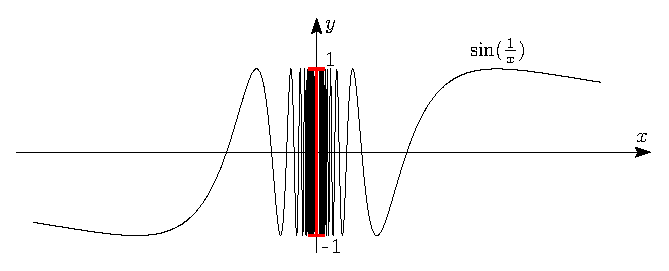
\includegraphics[width=0.75\textwidth]{11_1.eps}
	\caption{Связное множество $X$, которое не является линейно связным.}
	\label{11_1}
\end{figure}
Рассмотрим следующее множество 
$$
	X = \{\,(x, \sin{\tfrac{1}{x}}) \in \MR^2 \mid x \neq 0 \,\} \cup \{\, (0,y) \in 	\MR^2  \mid -1 \leq y \leq 1 \,\}
$$
\begin{exrc}
	Проверить, что это множество $X$ на плоскости $\MR^2$ связно, но не является линейно связным.
\end{exrc}
\begin{proof}
	Для начала рассмотрим следующую лемму.
	\begin{lemma}
		Пусть $X, Y$ - связные подмножества, $X \cap Y \neq \VN$, тогда $X \cup Y$ - связное подмножество того же пространства.
	\end{lemma}
	\begin{proof}
		(От противного) Пусть $Z = X \cup Y$ - несвязное множество, тогда $\exists$ открытые множества $U,V$ такие, что:
		$$
			Z \cap U \neq \VN,\, Z \cap V \neq \VN, \, U \cap V = \VN, \, Z \subset U \cup V
		$$
		Пусть $x \in X \cap Y \Rightarrow x \in U \vee x \in V$, пусть $x \in U$, поскольку множество $Z \cap V \neq \VN \Rightarrow \exists \, y \in V \colon y \in X \cup Y$. При этом $x \in X \wedge x \in Y \Rightarrow$ пусть $y \in Y$, тогда $y \in V \cap Y$ и одновременно с этим $x \in U \cap Y$. Получаем, что:
		$$
			Y \cap U \neq \VN, \, Y \cap V \neq \VN, \, U \cap V = \VN,\, Y \subset U \cup V 
		$$ 
		противоречие с тем, что $Y$ - связное множество. Аналогично, если $x \in V$ и аналогично для $y \in X$.
	\end{proof}
	Рассмотрим $X$ как составленное из следующих множеств:
	$$
		V = \{\, (0,y) \in 	\MR^2  \mid -1 \leq y \leq 1 \,\}, \, U_+ = \{\,(x, \sin{\tfrac{1}{x}}) \in \MR^2 \mid x > 0 \,\}, \, U_- = \{\,(x, \sin{\tfrac{1}{x}}) \in \MR^2 \mid x < 0 \,\}
	$$
	$$
		X = V \cup U_+ \cup U_{-} \subset \MR^2
	$$
	\begin{prop}
		Множество $V \cup U_{+}$ является связным подмножеством $\MR^2$.
	\end{prop}
	\begin{proof}
		Каждое множество по отдельности $V$ и $U_+$ являются линейно связным множеством $\Rightarrow$ это связные множества. Предположим, что $Y = V \cup U_+$ - не является связным, тогда $\exists$ открытые множества $S, P$ такие, что:
		$$
			S \neq \VN,\, P \neq \VN, \, S \cap P = \VN, \, Y = S \cup P
		$$
		Поскольку несвязность как подмножества, так и метрического пространства это одно и то же. По замечаниию выше $S, P$ - являются одновременно открытыми и замкнутыми множествами, тогда множества $S \cap U_+,\, P \cap U_+$ - также являются открытыми в $U_+$, по утверждению доказанному ранее. Тогда: 
		$$
			U_+ = Y \cap U_+ = (S \cup P) \cap U_+ = (S \cap U_+) \cup (P \cap U_+), \, (S \cap U_+) \cap (P \cap U_+) = \VN
		$$
		Тогда $U_+$ лежит в одном из множеств $S$ или $P$, иначе оно несвязно $\Rightarrow$ пусть $U_+ \subset S$. По аналогичным рассуждениям, $V$ лежит в $P$, в противном случае оно несвязно или $Y \cap P = \VN \Rightarrow P = \VN$. 
		
		Пусть $(0,y_0) \in V \colon \sin{(u)} = y_0$. Поскольку $\sin{(u + 2\pi n)} = y_0$, то мы можем предположить, что $u > 0$ и пусть $x_n = \tfrac{1}{u+ 2 \pi n}$, тогда: 
		$$
			(x_n, y_n) = (x_n, \sin{(\tfrac{1}{x_n})}) = (\tfrac{1}{u + 2\pi n},y_0) \in U_+, \, (x_n, y_n) \to (0, y_0) \in V
		$$
		Поскольку $S$ это замкнутое множество в $Y$, то оно должно содержать все пределы последовательностей в $S$, в том числе и для $U_+ \subset S \Rightarrow V \subset S$, в силу произвольности $(0,y_0) \in V$.
		Таким образом получили, что множество $P = \VN \Rightarrow$ противоречие $\Rightarrow Y = V \cup U_+$ - связное.
	\end{proof}
	Аналогично $V \cup U_{-}$ - связное множество и пересечение не пусто: $(U_- \cup V) \cap (U_+ \cup V) = V$, так как $U_- \cap U_+ = \VN$.
	По лемме выше, объединение этих двух множеств $X = (U_- \cup V) \cup (U_+ \cup V) = U_- \cup U_+ \cup V$ даст связное множество. Покажем, что $V \cup U_+$ не является линейно связным множеством.
	\begin{prop}
		Множество $Z = V \cup U_+$ не является линейно связным множеством.
	\end{prop}
	\begin{proof}
		(От противного) Пусть множество $Z$ является линейно связным, тогда $\forall (x_0, y_0), (x_1,y_1) \in Z, \, \exists$ кривая:
		$$
			g \colon [0,1] \to Z \colon g(0) = (x_0,y_0), g(1) = (x_1,y_1)
		$$ 
		Пусть $g(0) \in V, g(1) \in U_+$, поскольку множество $V$ - замкнуто, то $g^{-1}(V)$ - также будет замкнуто по непрерывности $g$, а поскольку оно еще и ограниченно, то по теореме Вейрштрасса:
		$$
			\exists \, c \in g^{-1}(V) \colon \forall t \in g^{-1}(V) \subset [0,1], \, c \geq t
		$$ 
		Переопределим функцию так, чтобы $f(t) = g(c + t(1-c))$, тогда $f(0) \in V,  \, f(t) \in U_+, \, \forall t \in (0,1]$. Очевидно, что $x(0) = 0$ и поскольку $f(t) = (x(t),y(t))$ - непрерывная функция $\Rightarrow x(t), y(t)$ - непрерывные функции. Для любого $n \geq 1$ выберем значение $u_2 \colon u_2 > \tfrac{1}{x(\tfrac{1}{n})}$ так, чтобы $\sin{(u_2)} = (-1)^n$. 
		
		Пусть $x_2 = \tfrac{1}{u_2} \Rightarrow 0 = x(0) < x_2  < x(\tfrac{1}{n})$ и при этом $\sin(\tfrac{1}{x_2}) = \sin{(u_2)} = (-1)^n$. По теореме о промежуточном значении $\exists \, t_n \in (0, \tfrac{1}{n}) \colon x(t_n) = x_2$. Тогда получим:
		$$
			0 < t_n < \tfrac{1}{n} \Rightarrow t_n \to 0 \Rightarrow x(t_n) \to x(0) = 0, \, y(t_n) = \sin{(\tfrac{1}{x_n})} = (-1)^n \nrightarrow y(0)
		$$
		Получили противоречие с непрерывностью $y(t)$.
	\end{proof}
	Вместо множества $V$ мы можем взять множество $U_- \cup V$, и проделать аналогичные рассуждения, что в любом случае приведет к тому, что $X$ - линейно несвязное множество.
\end{proof}
	
В общем случае условие линейной связности в метрическом пространстве - достаточное, но не необходимое. В нормированном пространстве возможна равносильность при наличии открытости множества.

\begin{prop}
	Если $E$ - открытое и связное множество в нормированном пространстве $(X,\|\cdot\|)$, то $E$ - линейно связно.
\end{prop}
\begin{proof}
	Введем на $E$ отношение эквивалентности: $x \sim y, \, x, y \in E$, если $x$ можно соединить с $y$ кривой, содержащейся в $E$. Проверим выполнение свойств эквивалентности:
	\begin{enumerate}[label ={(\arabic*)}]
		\item $\forall x_0 \in E, \, x_0 \sim x_0 \Leftrightarrow x(t) \equiv x_0$ (рефлексивность);
		
		\item $\forall x_0, x_1 \in E,\, x_0 \sim x_1 \Leftrightarrow \exists \, x(t) \colon x(0) = x_0, \, x(1) = x_1 \Leftrightarrow \exists \, x(1-t) \colon x(1) = x_0, \, x(0) = x_1 \Leftrightarrow x_1 \sim x_0$, таким образом $\forall x_0, x_1 \in E,\, x_0 \sim x_1 \Leftrightarrow x_1 \sim x_0$ (симметричность);
		
		\item $\forall x_0, x_1, x_2 \in E \colon x_0 \sim x_1 \wedge x_1 \sim x_2 \Leftrightarrow \exists \, x(t) \colon x(0) = x_0, \, x(1) = x_1 \wedge \exists \, \widetilde{x}(t)\colon \widetilde{x}(0) = x_1, \, \widetilde{x}(1) = x_2 \Rightarrow$ возьмем следующую кривую $g(t) = x(2t), \, t \in [0,\tfrac{1}{2}], \, g(t) = \widetilde{x}(2t-1), \,  t \in [\tfrac{1}{2},1]$, она непрерывна, поскольку она непрерывна на отрезках $[0,\tfrac{1}{2}], \, [\tfrac{1}{2},1]$ и верно следующее: 
		$$
			x(2{\cdot}\tfrac{1}{2}) = x(1) = x_1 = \widetilde{x}(2{\cdot}\tfrac{1}{2}-1) = \widetilde{x}(0) = g(\tfrac{1}{2})
		$$
		Одновременно с этим: 
		$$
			g(0) = x(2{\cdot}0) = x_0, \, g(1) = \widetilde{x}(2{\cdot}1-1) = \widetilde{x}(1) = x_2 
		$$
		Как результат, мы получили непрерывную кривую в $E$, соединяющую $x_0$ и $x_2 \Rightarrow$ таким образом верно, что $\forall x_0, x_1, x_2 \in E \colon x_0 \sim x_1 \wedge x_1 \sim x_2 \Rightarrow x_0 \sim x_2$ (транзитивность);
	\end{enumerate}
	Тогда множество $E = $ объединению попарно непересекающихся классов эквивалентности. Класс эквивалентности множества $E$ с представителем $x_0$ это $E_{x_0} = \{\,x \in X \mid x \sim x_0 \,\}$. 
	\begin{figure}[H]
		\centering
		\includegraphics[width=0.25\textwidth]{11_2.eps}
		\caption{Классы эквивалентностей точек $x_0$ и $x_1$.}
		\label{11_2}
	\end{figure}
	Если число классов эквивалентности равно $1$, то $E$ - линейно связно. $E_{x_0}$ - открытое множество, покажем это. Пусть $x \in E_{x_0} \Rightarrow$ существует непрерывная кривая из $x_0$ в точку $x$. 

	Поскольку $E$ - открытое, то $\forall x \in E, \, \exists \, B(x,r) \subset E $. Тогда из точки $x$ до любой точки $y \in B(x,r)$ существует прямая $x(t) = x + t(y -x), \, t\in [0,1]$ все точки которой принадлежат шару $B(x,r)$, поскольку пространство нормированное: 
	$$
		\forall y \in B(x,r), \, \exists \, x(t) = x + t(y -x) \colon \forall t \in [0,1], \, x(t) \in B(x,r)
	$$
	\begin{figure}[H]
		\centering
		\includegraphics[width=0.55\textwidth]{11_3.eps}
		\caption{Соединение точек шара $B(x,r)$ и точки $x$ через прямую $x(t) = x + t(y-x) \in B(x,r)$.}
		\label{11_3}
	\end{figure}
	Таким образом, любая точка $y \in B(x,r)$ соединяется отрезком с точкой $x \Rightarrow B(x,r) \subset E_{x_0}$, следовательно множество $E_{x_0}$ - открыто. 
	
	Если число классов эквивалентностей больше $1$, то $E$ распадается в объединение двух непустых, непересекающихся открытых множеств, что противоречит связности $E$.	
\end{proof}
\begin{defn}
	Функция $f \colon X \to Y$ - \uwave{гомеоморфизм}, если $f$ - биекция и $f,f^{-1}$ - непрерывны.
\end{defn}
\begin{exrc}
	Существует ли гомеоморфизм:
	\begin{figure}[H]
		\centering
		\begin{subfigure}[c]{0.5\textwidth}
			\centering
			\includegraphics{11_4.eps}
			\caption{Отрезка и квадрата.}
			\label{fig:11_4}
		\end{subfigure}
		\begin{subfigure}[c]{0.49\textwidth}
			\centering
			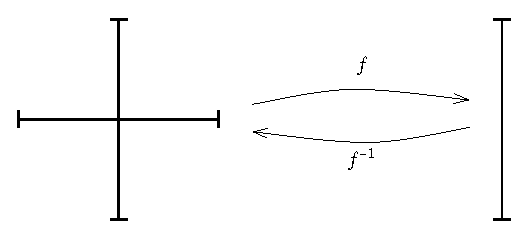
\includegraphics{11_5.eps}
			\caption{Пересечения отрезков и отрезка.}
			\label{fig:11_5}
		\end{subfigure}
		\caption{Существование гомеоморфизмов.}	
		\label{fig:Гомеоморфизм}
	\end{figure}
	\begin{enumerate}[label ={\arabic*)}]
		\item Отрезка и квадрата?
		\item Двух пересекающихся отрезков и отрезка?
	\end{enumerate}
\end{exrc}
\begin{proof}
	В обоих случаях предположим, что гомеоморфизм существует. По определению гомеоморфизм это непрерывная биекция с непрерывной обратной функцией. Таким образом функция инъективна и если мы выбросим одну точку из области определения и области значения, гомеоморфзим сохранится. Функция и обратная функция останутся непрерывными, проверим свойства связности у данных множеств.
	\begin{figure}[H]
		\centering
		\begin{subfigure}[c]{0.5\textwidth}
			\centering
			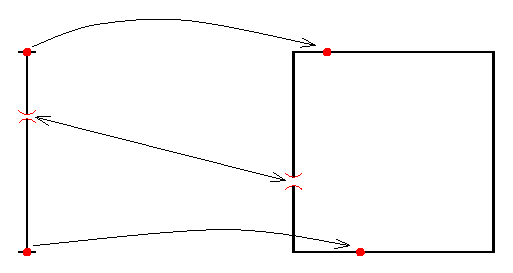
\includegraphics{11_6.eps}
			\caption{Отрезка и квадрата.}
			\label{fig:11_6}
		\end{subfigure}
		\begin{subfigure}[c]{0.49\textwidth}
			\centering
			\includegraphics{11_7.eps}
			\caption{Пересечения отрезков и отрезка.}
			\label{fig:11_7}
		\end{subfigure}
		\caption{Отсутствие гомеоморфизмов.}	
		\label{fig:Гомеоморфизм}
	\end{figure}
	\begin{enumerate}[label ={\arabic*)}]
		\item Очевидно, если убрать концевые точки отрезка, он останется линейно связным множеством. Квадрат это линейно связное множество $\Rightarrow$ связное множество. Если убрать из квадрата любую точку, он все равно останется связным множеством. 
		
		Уберем точку $a$ из середины отрезка и уберем соответствующую ей точку $f(a)$ из квадрата. Квадрат остался связным множеством, тогда как отрезок стал несвязным. Поскольку $f^{-1}$ - непрерывная функция и $Y \setminus \{f(a)\}$ - связное множество, то $f^{-1}(Y \setminus \{f(a)\}) = X \setminus \{a\}$ должно быть связным, но это не так $\Rightarrow$ получили противоречие.
		\item Пересечение отрезков - связное множество, если хотя бы одна концевая точка пересекающихся отрезков отображается внутрь отрезка, то убрав такую точку и её отображение, пересечение отрезков останется связным множеством, тогда как отрезок станет несвязным. 
		
		Поскольку $f$ - биекция, то она инъективна и значит, что хотя бы две концевые точки пересекающихся отрезков будут отображаться внутрь отрезка. Мы получили противоречие поскольку $f$ непрерывная, а образ связного множества должен быть связным. 
	\end{enumerate}
\end{proof}

\begin{exrc}
	Доказать, что, если в $\MR^n$ есть два базиса с матрицей перехода $A, \, \det{A} > 0$, то существует непрерывное преобразование одного базиса в другой.
\end{exrc}
\begin{proof}
	Будем использовать метод исключения переменных (метод Гаусса), чтобы связать любую матрицу перехода $A, \, \det{A} > 0$ с единичной матрицей $I_n$. Рассмотрим следующую матрицу, элементы которой совпадают с единичной матрицей, за исключением одного $(i,j)$-го элемента, расположенного вне диагонали:
	$$
		I_{i,j}(r) = I_n + rP_{i,j}, \, r \in \MR
	$$
	$$
		P_{i,j} = (\delta_{kl}(i,j)),\, 1 \leq i \neq j \leq n, \, \delta_{kl}(i,j) = \begin{cases}
			1, & k = i \wedge l = j\\
			0, & k \neq i \vee l \neq j
		\end{cases}
	$$
	Таким образом, домножение матрицы $I_{i,j}(r)$ на любую матрицу $A$ слева даст сложение  домноженной на скаляр $r$ строки $j$ матрицы $A$ к строке $i$. Следовательно, следующее отображение:
	$$
		f\colon [0,1] \to \MR^{n^2}, \,  f(t) = I_{i,j}(tr)A, \, t \in [0,1]
	$$
	определеяет непрерывный путь из матрицы $A$ к матрице $I_{i,j}(r)A$. Используя эту операцию можно определить операцию перестановки строк с изменением знака:
	$$
		I_{j,i}(1){\cdot}I_{i,j}(-1){\cdot}I_{j,i}(1)
	$$
	Если рассматривать пересечение $i,j$-ых столбцов и $i,j$-ых строк этого выражения, то получим следующие подматрицы:
	$$
		\begin{pmatrix}
			1 & 0 \\
			1 & 1
		\end{pmatrix}{\cdot}
		\begin{pmatrix}
			1 & -1 \\
			0 & \phantom{-}1
		\end{pmatrix}{\cdot}
		\begin{pmatrix}
			1 & 0 \\
			1 & 1
		\end{pmatrix} = 
		\begin{pmatrix}
			\phantom{-}0 & 1 \\
			-1 & 0
		\end{pmatrix}
	$$
	Следовательно, если матрица $B$ получена из матрицы $A$ перестановкой строк с изменением знака, то между ними существует непрерывное преобразование. 
	
	Используя операции выше, мы можем создать непрерывный путь, который будет соединить любую обратимую матрицу $A$ и диагональную матрицу $D$ вида:
	$$
		D = \text{diag}\{d_1,d_2, \dotsc, d_n\} = 
		\begin{pmatrix}
			d_1 & 0 & \dotsc & 0 \\
			0 & d_2 & \dotsc & 0\\
			\vdots & \vdots & \ddots & \vdots \\
			0 & 0 & \dotsc & d_n
		\end{pmatrix}, \, d_i \neq 0, \, \forall i = \overline{1,n}
	$$
	Если $d_i$ и $d_j$ отрицательны для $i \neq j$, тогда можно переставить строки $i$ и $j$ дважды (каждый раз меняя знак: $d_i \to -d_i, \, d_j \to - d_j$). Таким образом, мы получим таблицу, где отрицательным может быть только один элемент. Также заметим, что $\det{D} = d_1 d_2 \dotsc d_n$ и если он положителен, то все элементы также будут положительными. Но поскольку приведение к такому виду не изменяло определитель (перестановка строк со сменой знака, прибавление к строке другой строки, умноженной на скаляр), то $\det{A} = \det{D} > 0 \Rightarrow$ все элементы положительные.
	
	Последняя операция, которую мы определим - домножение на ненулевой скаляр $r \in (0,\infty)$ строки $i$. Эта операция в матричном виде выражается в домножении слева на диагональную матрицу:
	$$
		S(i,r) = \text{diag}(1,\dotsc,1,r,1,\dotsc,1)
	$$
	которая отличается от $I_n$ только элементом в $i$-ой строчке, равному $r$. И таким образом для $r > 0$ следующий путь:
	$$
		g \colon [0,1] \to \MR^{n^2}, \, g(t) = \text{diag}(1,\dotsc,1,(1-t) + tr,1,\dotsc,1)A = S(i,(1-t) + tr)A, \, t \in [0,1]
	$$
	непрерывно соединяет матрицу $A$ с матрицей $S(i,r)A$. Применяя последовательно эту операцию к полученной матрице $D$ с коэффициентами $r = \dfrac{1}{d_i}$ для каждой строки $1 \leq i \leq n$, мы получим непрерывный путь, соединяющий исходную матрицу $A, \, \det{A} >0$ с единичной матрицей $I_n$. Таким образом, получили непрерывное преобразование из одного базиса в другой.
\end{proof}

\begin{exrc}
	$GL(n,\MR) = \{\,A \mid \det{A} \neq 0 \,\} \subset \MR^{n^2}$ - полная линейная группа, состоит из всех обратимых матриц. Доказать, что $GL_+(n,\MR) = \{\,A \mid \det{A} > 0 \,\}$ - линейно связное множество.
\end{exrc}
\begin{proof}
	Следует сразу из предыдущей задачи. Поскольку любая матрица внутри множества $GL_+(n,\MR)$ может быть приведена к единичной $\Rightarrow$ можно через неё связать все остальные матрицы $\Rightarrow$ множество линейно связно.
\end{proof}

\begin{exrc}
	Доказать, что $SL(n,\MR) = \{\,A \mid \det{A} = 1 \,\}$ является линейно связным множеством.
\end{exrc}
\begin{proof}
	Используя следующее непрерывное преобразование для всех матриц $A, \det{A} > 0$:
	$$
		h \colon \MR^{n^2} \to \MR^{n^2}, \, h(A) = \dfrac{1}{\sqrt[n]{\det{A}}}A, \, \det{(h(A))} = \bigg( \dfrac{1}{\sqrt[n]{\det{A}}}\bigg)^n {\cdot}\det{A} = 1
	$$	
	и используя результат упражнения выше, получаем, что любые матрицы в $SL(n,\MR)$ могут быть непрерывно преобразованы в $I_n \Rightarrow$ множество является линейно связным.
\end{proof}

\newpage
\section*{Линейные функции}
Пусть $X$ и $Y$ - нормированные пространства.
\begin{defn}
	Отображение $L \colon X \to Y$ называется \uwave{линейным} (или еще говорят линейным оператор), если выполнено следующее: 
	$$
		L(\alpha_1 x_1 + \alpha_2 x_2) = \alpha_1 L(x_1) + \alpha_2 L(x_2)
	$$ 
\end{defn}

\subsection*{Конечномерные линейные отображения}
\textbf{Пример}: Возникает вопрос, как например устроено $L \colon \MR \to \MR$? Возьмем базисный вектор $e_1 = 1$, тогда: 
$$
	x = x_1 e_1 = x_1 \Rightarrow L(x) = L(x_1 e_1) = x_1L(e_1) = x L(e_1) = kx
$$
\textbf{Пример}: Как устроено линейное отображение $L\colon \MR^n \to \MR$ (\uwave{линейный функционал})? Возьмем базис пространства $\MR^n$: $e_1,\dotsc e_n \Rightarrow$ любой элемент $x$ представится в виде $x = x_1 e_1 + \dotsc + x_n e_n$, тогда:
$$
	L(x) = x_1 L(e_1) + \dotsc + x_n L(e_n) = a_1 x_1 + \dotsc + a_n x_n
$$
\textbf{Пример}: Как устроено линейное отображение $L\colon \MR^n \to \MR^m$? Возьмем базис пространства $\MR^n$: $e_1,\dotsc e_n \Rightarrow$ любой элемент $x$ представится в виде $x = x_1 e_1 + \dotsc + x_n e_n$, тогда:
$$
	L(x) = x_1 L(e_1) + \dotsc + x_n L(e_n), \, 
	L(e_1) = \begin{pmatrix}
		a_{11}\\
		a_{21}\\
		\vdots\\
		a_{m1}
	\end{pmatrix}, \dotsc,
	L(e_n) = \begin{pmatrix}
		a_{1n}\\
		a_{2n}\\
		\vdots\\
		a_{mn}
	\end{pmatrix} \Rightarrow
$$
$$
	\Rightarrow L(x) = x_1 L(e_1) + \dotsc + x_n L(e_n) = 
	\overbrace{\begin{pmatrix}
		a_{11} & \dotsc & a_{1n}\\
		a_{21} & \dotsc & a_{2n}\\
		\vdots & \ddots & \vdots\\
		a_{m1} & \dotsc & a_{mn}
	\end{pmatrix}}^{A}{\cdot}
	\overbrace{\begin{pmatrix}
		x_1\\
		x_2\\
		\vdots\\
		x_n
	\end{pmatrix}}^{X} = A{\cdot}X
$$
Очевидно, что $L$ - непрерывное отображение, поскольку везде это арифметические операции с непрерывными функциями $x_1,\dotsc, x_n$. Но в общем случае, линейное отображение может быть разрывной функцией.

\subsection*{Бесконечномерные линейные отображения}
\textbf{Пример}: Возьмем пространство непрерывных дифференцируемых функций $C^1[0,1]$ с нормой максимума функции: $\|f\| = \max\limits_t |f(t)|$. Рассмотрим следующее линейное отображение: 
$$
	L\colon C^1[0,1] \to \MR,\, L(f) = f^\prime(0)
$$
Легко проверить, что оно действительно является линейным:
$$
	L(\alpha f + \beta g) = (\alpha f + \beta g)^\prime(0) = \alpha f^\prime(0) + \beta g^\prime(0) = \alpha L(f) + \beta L(g)
$$
Но при этом, оно не является непрерывным. Например, $f_n(x) = \frac{1}{n}\sin{(n^2x)}$, тогда:
$$
	0 \leq f_n \leq \tfrac{1}{n}, \, f_n \rightrightarrows 0, \, L(f_n) = f_n^\prime(0) = n \to \infty, \, L(f_n) \nrightarrow L(0)
$$
В конечномерном пространстве линейный функционал всегда непрерывен, но в бесконечномерном пространстве всегда найдется линейный функционал, который будет разрывным.
\begin{rem}
	Пример на полном пространстве придумать сложнее, но там можно воспользоваться базисом Гамеля и аксиомой выбора.
\end{rem}

С точки зрения анализа полезно понять, какие достаточные условия непрерывности на линейные функции надо накладывать. 

\begin{theorem}
	Пусть $L\colon X \to Y$ - линейная функция, тогда следующие утверждения равносильны:
	\begin{enumerate}[label ={(\arabic*)}]
		\item $L$ - непрерывна;
		\item $L$ - непрерывна в $0$;
		\item $\exists \, C > 0 \colon \|L(x)\|_Y \leq C \|x\|_X, \, \forall x$;
	\end{enumerate}
\end{theorem}

\end{document}